\section{Deployment View}

The SafeStreets platform can be divided into the following Tiers that separate different aspects of the application.
\begin{itemize}
  \item Client: it represents the client application. It will be the Web Application running in the browser or the native mobile application running on the target OS
  \item Reverse Proxy: it represents the intermediary between the client and the server application. It will provide basic functionalities such as data compression and caching.
  \item Server Application: it represents both the static file serving service and the application that provides the REST APIs for accessing and creating dynamic information
  \item Database: it represents the data storage solution. This tier identifies both the RDBMS and the media storage
\end{itemize}


This is more of a logical separation due to the fact that we'll be using a Cloud Infrastructure Provider, thus the real architecture may vary
based on the specific company offering the service.
\newline
\newline
In the following page a simplified graphical representation of the architecture previously described is provided.
\newpage

\begin{figure}[H]
  \centering
  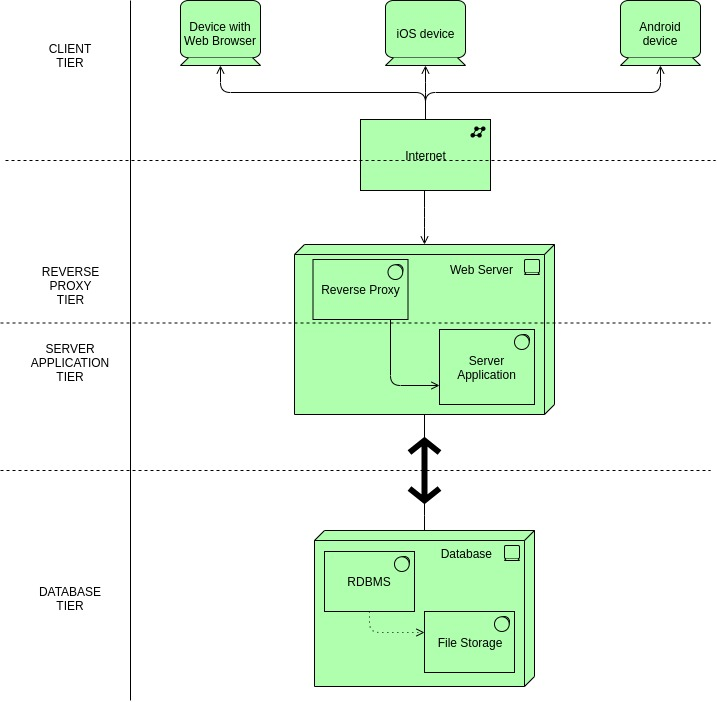
\includegraphics[origin=c,width=\textwidth,height=.95\textheight,keepaspectratio]{DD_Images/DeploymentView.jpg}
  \caption{\textit{Simplified Architecture diagram}}
\end{figure}